% Options for packages loaded elsewhere
\PassOptionsToPackage{unicode}{hyperref}
\PassOptionsToPackage{hyphens}{url}
%
\documentclass[
]{article}
\usepackage{lmodern}
\usepackage{amssymb,amsmath}
\usepackage{ifxetex,ifluatex}
\ifnum 0\ifxetex 1\fi\ifluatex 1\fi=0 % if pdftex
  \usepackage[T1]{fontenc}
  \usepackage[utf8]{inputenc}
  \usepackage{textcomp} % provide euro and other symbols
\else % if luatex or xetex
  \usepackage{unicode-math}
  \defaultfontfeatures{Scale=MatchLowercase}
  \defaultfontfeatures[\rmfamily]{Ligatures=TeX,Scale=1}
\fi
% Use upquote if available, for straight quotes in verbatim environments
\IfFileExists{upquote.sty}{\usepackage{upquote}}{}
\IfFileExists{microtype.sty}{% use microtype if available
  \usepackage[]{microtype}
  \UseMicrotypeSet[protrusion]{basicmath} % disable protrusion for tt fonts
}{}
\makeatletter
\@ifundefined{KOMAClassName}{% if non-KOMA class
  \IfFileExists{parskip.sty}{%
    \usepackage{parskip}
  }{% else
    \setlength{\parindent}{0pt}
    \setlength{\parskip}{6pt plus 2pt minus 1pt}}
}{% if KOMA class
  \KOMAoptions{parskip=half}}
\makeatother
\usepackage{xcolor}
\IfFileExists{xurl.sty}{\usepackage{xurl}}{} % add URL line breaks if available
\IfFileExists{bookmark.sty}{\usepackage{bookmark}}{\usepackage{hyperref}}
\hypersetup{
  pdftitle={Lab 9},
  pdfauthor={Zachary Palmore},
  hidelinks,
  pdfcreator={LaTeX via pandoc}}
\urlstyle{same} % disable monospaced font for URLs
\usepackage[margin=1in]{geometry}
\usepackage{color}
\usepackage{fancyvrb}
\newcommand{\VerbBar}{|}
\newcommand{\VERB}{\Verb[commandchars=\\\{\}]}
\DefineVerbatimEnvironment{Highlighting}{Verbatim}{commandchars=\\\{\}}
% Add ',fontsize=\small' for more characters per line
\usepackage{framed}
\definecolor{shadecolor}{RGB}{248,248,248}
\newenvironment{Shaded}{\begin{snugshade}}{\end{snugshade}}
\newcommand{\AlertTok}[1]{\textcolor[rgb]{0.94,0.16,0.16}{#1}}
\newcommand{\AnnotationTok}[1]{\textcolor[rgb]{0.56,0.35,0.01}{\textbf{\textit{#1}}}}
\newcommand{\AttributeTok}[1]{\textcolor[rgb]{0.77,0.63,0.00}{#1}}
\newcommand{\BaseNTok}[1]{\textcolor[rgb]{0.00,0.00,0.81}{#1}}
\newcommand{\BuiltInTok}[1]{#1}
\newcommand{\CharTok}[1]{\textcolor[rgb]{0.31,0.60,0.02}{#1}}
\newcommand{\CommentTok}[1]{\textcolor[rgb]{0.56,0.35,0.01}{\textit{#1}}}
\newcommand{\CommentVarTok}[1]{\textcolor[rgb]{0.56,0.35,0.01}{\textbf{\textit{#1}}}}
\newcommand{\ConstantTok}[1]{\textcolor[rgb]{0.00,0.00,0.00}{#1}}
\newcommand{\ControlFlowTok}[1]{\textcolor[rgb]{0.13,0.29,0.53}{\textbf{#1}}}
\newcommand{\DataTypeTok}[1]{\textcolor[rgb]{0.13,0.29,0.53}{#1}}
\newcommand{\DecValTok}[1]{\textcolor[rgb]{0.00,0.00,0.81}{#1}}
\newcommand{\DocumentationTok}[1]{\textcolor[rgb]{0.56,0.35,0.01}{\textbf{\textit{#1}}}}
\newcommand{\ErrorTok}[1]{\textcolor[rgb]{0.64,0.00,0.00}{\textbf{#1}}}
\newcommand{\ExtensionTok}[1]{#1}
\newcommand{\FloatTok}[1]{\textcolor[rgb]{0.00,0.00,0.81}{#1}}
\newcommand{\FunctionTok}[1]{\textcolor[rgb]{0.00,0.00,0.00}{#1}}
\newcommand{\ImportTok}[1]{#1}
\newcommand{\InformationTok}[1]{\textcolor[rgb]{0.56,0.35,0.01}{\textbf{\textit{#1}}}}
\newcommand{\KeywordTok}[1]{\textcolor[rgb]{0.13,0.29,0.53}{\textbf{#1}}}
\newcommand{\NormalTok}[1]{#1}
\newcommand{\OperatorTok}[1]{\textcolor[rgb]{0.81,0.36,0.00}{\textbf{#1}}}
\newcommand{\OtherTok}[1]{\textcolor[rgb]{0.56,0.35,0.01}{#1}}
\newcommand{\PreprocessorTok}[1]{\textcolor[rgb]{0.56,0.35,0.01}{\textit{#1}}}
\newcommand{\RegionMarkerTok}[1]{#1}
\newcommand{\SpecialCharTok}[1]{\textcolor[rgb]{0.00,0.00,0.00}{#1}}
\newcommand{\SpecialStringTok}[1]{\textcolor[rgb]{0.31,0.60,0.02}{#1}}
\newcommand{\StringTok}[1]{\textcolor[rgb]{0.31,0.60,0.02}{#1}}
\newcommand{\VariableTok}[1]{\textcolor[rgb]{0.00,0.00,0.00}{#1}}
\newcommand{\VerbatimStringTok}[1]{\textcolor[rgb]{0.31,0.60,0.02}{#1}}
\newcommand{\WarningTok}[1]{\textcolor[rgb]{0.56,0.35,0.01}{\textbf{\textit{#1}}}}
\usepackage{graphicx,grffile}
\makeatletter
\def\maxwidth{\ifdim\Gin@nat@width>\linewidth\linewidth\else\Gin@nat@width\fi}
\def\maxheight{\ifdim\Gin@nat@height>\textheight\textheight\else\Gin@nat@height\fi}
\makeatother
% Scale images if necessary, so that they will not overflow the page
% margins by default, and it is still possible to overwrite the defaults
% using explicit options in \includegraphics[width, height, ...]{}
\setkeys{Gin}{width=\maxwidth,height=\maxheight,keepaspectratio}
% Set default figure placement to htbp
\makeatletter
\def\fps@figure{htbp}
\makeatother
\setlength{\emergencystretch}{3em} % prevent overfull lines
\providecommand{\tightlist}{%
  \setlength{\itemsep}{0pt}\setlength{\parskip}{0pt}}
\setcounter{secnumdepth}{-\maxdimen} % remove section numbering

\title{Lab 9}
\author{Zachary Palmore}
\date{2020-11-20}

\begin{document}
\maketitle

\begin{Shaded}
\begin{Highlighting}[]
\KeywordTok{library}\NormalTok{(tidyverse)}
\KeywordTok{library}\NormalTok{(openintro)}
\end{Highlighting}
\end{Shaded}

\hypertarget{pre-exercise}{%
\subsubsection{Pre-exercise}\label{pre-exercise}}

Adding the GGally package.

\begin{Shaded}
\begin{Highlighting}[]
\CommentTok{# install.packages("GGally")}
\KeywordTok{library}\NormalTok{(GGally)}
\end{Highlighting}
\end{Shaded}

\begin{verbatim}
## Warning: package 'GGally' was built under R version 4.0.3
\end{verbatim}

\begin{verbatim}
## Registered S3 method overwritten by 'GGally':
##   method from   
##   +.gg   ggplot2
\end{verbatim}

Looking at the data from the course package.

\begin{Shaded}
\begin{Highlighting}[]
\KeywordTok{data}\NormalTok{(evals)}
\KeywordTok{glimpse}\NormalTok{(evals)}
\end{Highlighting}
\end{Shaded}

\begin{verbatim}
## Rows: 463
## Columns: 23
## $ course_id     <int> 1, 2, 3, 4, 5, 6, 7, 8, 9, 10, 11, 12, 13, 14, 15, 16...
## $ prof_id       <int> 1, 1, 1, 1, 2, 2, 2, 3, 3, 4, 4, 4, 4, 4, 4, 4, 4, 5,...
## $ score         <dbl> 4.7, 4.1, 3.9, 4.8, 4.6, 4.3, 2.8, 4.1, 3.4, 4.5, 3.8...
## $ rank          <fct> tenure track, tenure track, tenure track, tenure trac...
## $ ethnicity     <fct> minority, minority, minority, minority, not minority,...
## $ gender        <fct> female, female, female, female, male, male, male, mal...
## $ language      <fct> english, english, english, english, english, english,...
## $ age           <int> 36, 36, 36, 36, 59, 59, 59, 51, 51, 40, 40, 40, 40, 4...
## $ cls_perc_eval <dbl> 55.81395, 68.80000, 60.80000, 62.60163, 85.00000, 87....
## $ cls_did_eval  <int> 24, 86, 76, 77, 17, 35, 39, 55, 111, 40, 24, 24, 17, ...
## $ cls_students  <int> 43, 125, 125, 123, 20, 40, 44, 55, 195, 46, 27, 25, 2...
## $ cls_level     <fct> upper, upper, upper, upper, upper, upper, upper, uppe...
## $ cls_profs     <fct> single, single, single, single, multiple, multiple, m...
## $ cls_credits   <fct> multi credit, multi credit, multi credit, multi credi...
## $ bty_f1lower   <int> 5, 5, 5, 5, 4, 4, 4, 5, 5, 2, 2, 2, 2, 2, 2, 2, 2, 7,...
## $ bty_f1upper   <int> 7, 7, 7, 7, 4, 4, 4, 2, 2, 5, 5, 5, 5, 5, 5, 5, 5, 9,...
## $ bty_f2upper   <int> 6, 6, 6, 6, 2, 2, 2, 5, 5, 4, 4, 4, 4, 4, 4, 4, 4, 9,...
## $ bty_m1lower   <int> 2, 2, 2, 2, 2, 2, 2, 2, 2, 3, 3, 3, 3, 3, 3, 3, 3, 7,...
## $ bty_m1upper   <int> 4, 4, 4, 4, 3, 3, 3, 3, 3, 3, 3, 3, 3, 3, 3, 3, 3, 6,...
## $ bty_m2upper   <int> 6, 6, 6, 6, 3, 3, 3, 3, 3, 2, 2, 2, 2, 2, 2, 2, 2, 6,...
## $ bty_avg       <dbl> 5.000, 5.000, 5.000, 5.000, 3.000, 3.000, 3.000, 3.33...
## $ pic_outfit    <fct> not formal, not formal, not formal, not formal, not f...
## $ pic_color     <fct> color, color, color, color, color, color, color, colo...
\end{verbatim}

There are 463 rows and 23 columns.

Evaluating the type of study.

\begin{Shaded}
\begin{Highlighting}[]
\NormalTok{?evals}
\end{Highlighting}
\end{Shaded}

\begin{verbatim}
## starting httpd help server ... done
\end{verbatim}

\hypertarget{exercise-1}{%
\subsubsection{Exercise 1}\label{exercise-1}}

Is this an observational study or an experiment? The original research
question posed in the paper is whether beauty leads directly to the
differences in course evaluations. Given the study design, is it
possible to answer this question as it is phrased? If not, rephrase the
question.

This is an observational study because the data gathered is not directly
interfering with how the data arises and they are merely observing a
natural phenomena.

With an observational study, we cannot make causal claims. We can only
provide evidence that an association exists between two variables.

The question could be rephrased to ask, ``is there an association
between a professor's attractiveness and their course evaluations?''
which could be further broken down into a hypothesis test where:

\(H_o\) There is no relationship between a professor's attractiveness
and their course evaluations.

\(H_a\) There is a relationship between a professor's attractiveness and
their course evaluations.

It could then be tested to determine the validity of the association
between the variables.

\hypertarget{exercise-2}{%
\subsubsection{Exercise 2}\label{exercise-2}}

Describe the distribution of score. Is the distribution skewed? What
does that tell you about how students rate courses? Is this what you
expected to see? Why, or why not?

\begin{Shaded}
\begin{Highlighting}[]
\KeywordTok{hist}\NormalTok{(evals}\OperatorTok{$}\NormalTok{score, }\DataTypeTok{xlab =} \StringTok{"Score"}\NormalTok{, }\DataTypeTok{ylab =} \StringTok{"Counts"}\NormalTok{, }\DataTypeTok{main =} \StringTok{"Histogram of Scores"}\NormalTok{)}
\end{Highlighting}
\end{Shaded}

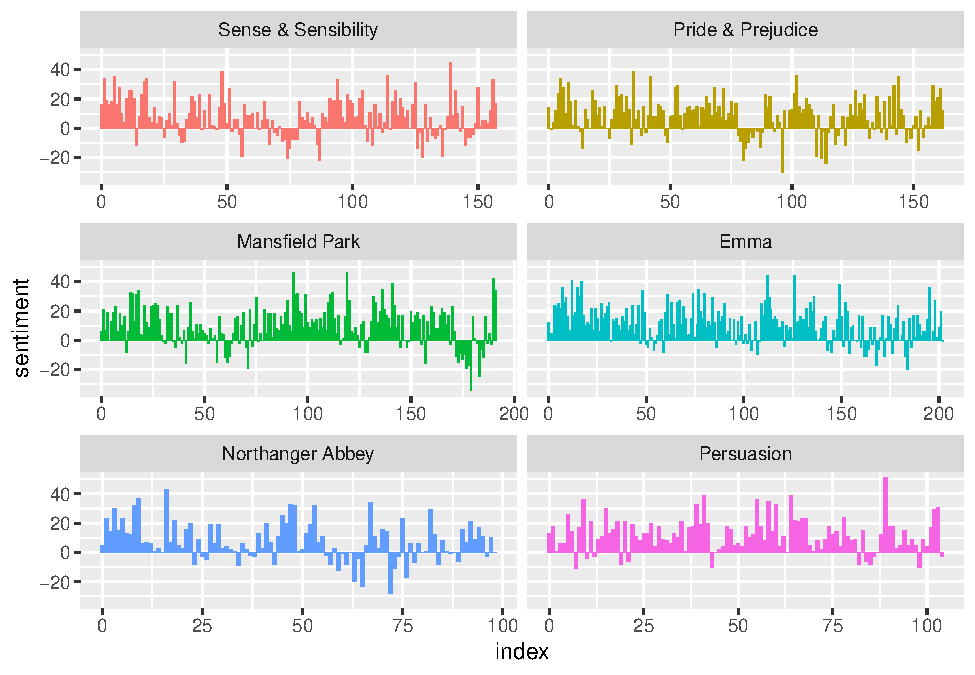
\includegraphics{Lab9_files/figure-latex/unnamed-chunk-4-1.pdf}

The expectation was a normal distribution (unimodal, bell-shaped around
the middle median/mean of 2.5) but this did not occur. The distribution
is left skewed which means students rated more positively. This means
that either the professors were all great and the random sample resulted
in higher numbers of positive ratings by chance, or something else is
going on here.

\hypertarget{exercise-3}{%
\subsubsection{Exercise 3}\label{exercise-3}}

Excluding score, select two other variables and describe their
relationship with each other using an appropriate visualization.

Two other variables are the average beauty score and ethnicity. Their
distributions are displayed in the boxplots below with the language of
the school where the professor received education as a third variable
for reference.

\begin{Shaded}
\begin{Highlighting}[]
\KeywordTok{ggplot}\NormalTok{(evals, }\KeywordTok{aes}\NormalTok{(bty_avg, ethnicity)) }\OperatorTok{+}\StringTok{ }\KeywordTok{geom_boxplot}\NormalTok{() }\OperatorTok{+}\StringTok{ }\KeywordTok{coord_flip}\NormalTok{() }\OperatorTok{+}\StringTok{ }\KeywordTok{theme_classic}\NormalTok{() }\OperatorTok{+}\StringTok{ }\KeywordTok{labs}\NormalTok{(}\DataTypeTok{x =} \StringTok{"Avg Score"}\NormalTok{, }\DataTypeTok{y =} \StringTok{"Ethnicity"}\NormalTok{, }\DataTypeTok{title =} \StringTok{"Average Beauty Scores by Ethnicity and Language"}\NormalTok{)}
\end{Highlighting}
\end{Shaded}

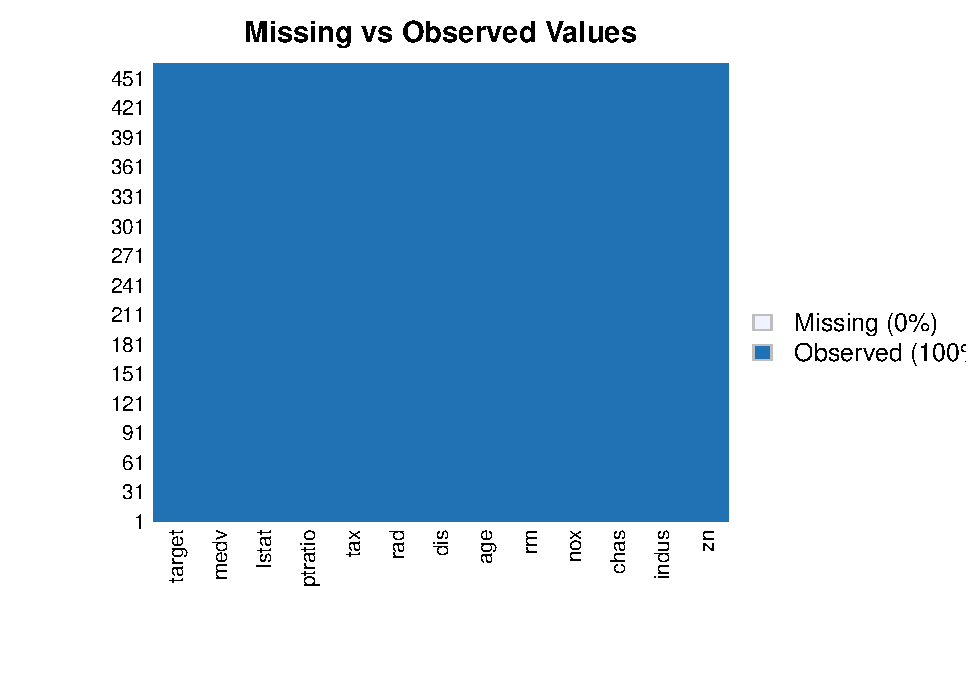
\includegraphics{Lab9_files/figure-latex/unnamed-chunk-5-1.pdf}

We can see the relationship between ethnicity and the average beauty
score is about the same between minorities and non-minorities. Their
interquartile range is also comparable but minority ethnicities are
slightly tighter in distribution than non-minorities. The outer range of
nonminorities is wider than minorities. I wonder if this would change if
we included new boxplots for professors who went to english and
non-english schools.

\begin{Shaded}
\begin{Highlighting}[]
\KeywordTok{ggplot}\NormalTok{(evals, }\KeywordTok{aes}\NormalTok{(bty_avg, ethnicity, }\DataTypeTok{fill =}\NormalTok{ language)) }\OperatorTok{+}\StringTok{ }\KeywordTok{geom_boxplot}\NormalTok{() }\OperatorTok{+}\StringTok{ }\KeywordTok{coord_flip}\NormalTok{() }\OperatorTok{+}\StringTok{ }\KeywordTok{theme_classic}\NormalTok{() }\OperatorTok{+}\StringTok{ }\KeywordTok{labs}\NormalTok{(}\DataTypeTok{x =} \StringTok{"Avg Score"}\NormalTok{, }\DataTypeTok{y =} \StringTok{"Ethnicity"}\NormalTok{, }\DataTypeTok{title =} \StringTok{"Average Beauty Scores by Ethnicity and Language"}\NormalTok{)}
\end{Highlighting}
\end{Shaded}

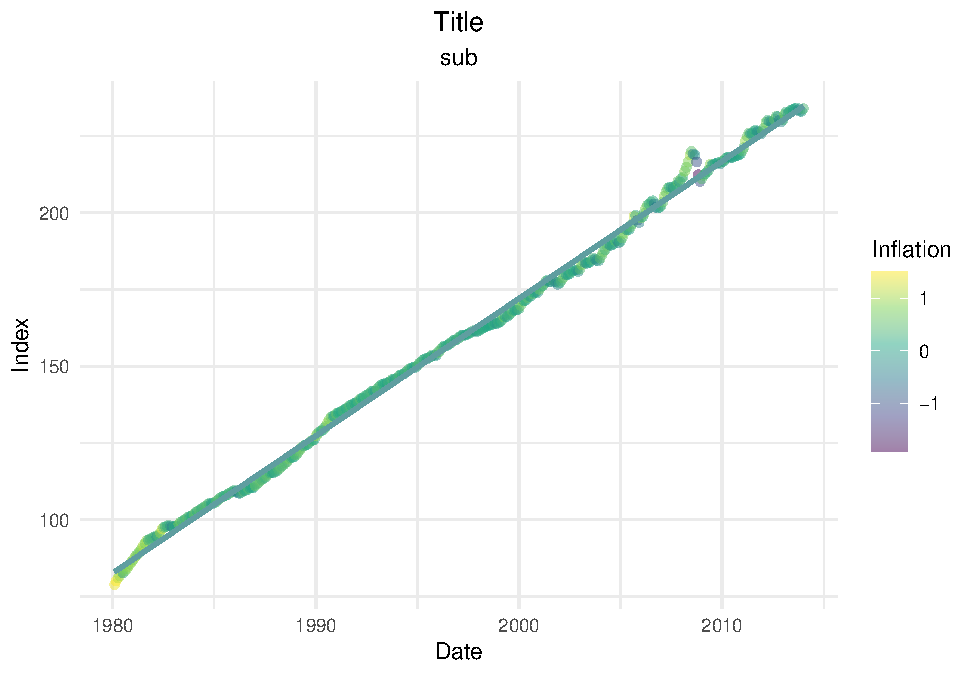
\includegraphics{Lab9_files/figure-latex/unnamed-chunk-6-1.pdf}

There is certainly a difference in distribution between the ethnicities
who's education was received in english and those who received an
education that was not in english. For example, minorities that had a
non-english education had higher beauty scores on average than those
whose education was in english. However, the results are different for
non-minorities. This group had an average very close to the average
score for all non-minorities that received an education in english.

\hypertarget{exercise-4}{%
\subsubsection{Exercise 4}\label{exercise-4}}

Replot the scatterplot, but this time use geom\_jitter as your layer.
What was misleading about the initial scatterplot?

The origional scatterplot is shown below.

\begin{Shaded}
\begin{Highlighting}[]
\KeywordTok{ggplot}\NormalTok{(}\DataTypeTok{data =}\NormalTok{ evals, }\KeywordTok{aes}\NormalTok{(}\DataTypeTok{x =}\NormalTok{ bty_avg, }\DataTypeTok{y =}\NormalTok{ score)) }\OperatorTok{+}
\StringTok{  }\KeywordTok{geom_point}\NormalTok{()}
\end{Highlighting}
\end{Shaded}

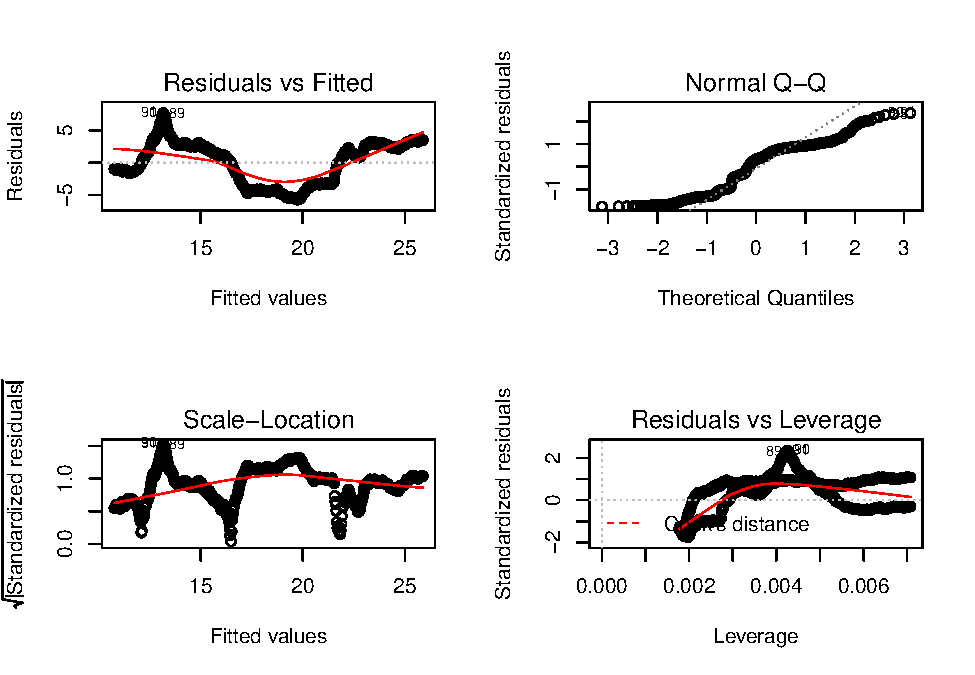
\includegraphics{Lab9_files/figure-latex/unnamed-chunk-7-1.pdf}

This is the recreation of the scatterplot using geom\_jitter.

\begin{Shaded}
\begin{Highlighting}[]
\KeywordTok{ggplot}\NormalTok{(}\DataTypeTok{data =}\NormalTok{ evals, }\KeywordTok{aes}\NormalTok{(}\DataTypeTok{x =}\NormalTok{ bty_avg, }\DataTypeTok{y =}\NormalTok{ score)) }\OperatorTok{+}
\StringTok{  }\KeywordTok{geom_jitter}\NormalTok{()}
\end{Highlighting}
\end{Shaded}

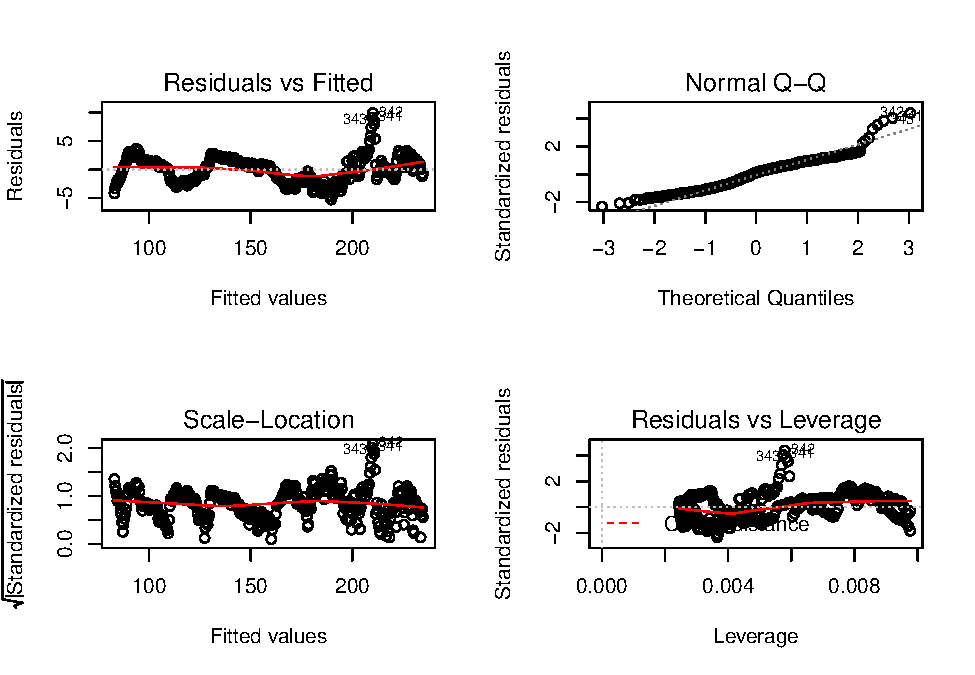
\includegraphics{Lab9_files/figure-latex/unnamed-chunk-8-1.pdf}

\begin{Shaded}
\begin{Highlighting}[]
\NormalTok{?geom_point}
\NormalTok{?geom_jitter}
\end{Highlighting}
\end{Shaded}

It appears as though the initial scatterplot was missing some points.
Looking into the geom\_point and geom\_jitter functions, we can see why.
The geom\_jitter function adds a small amount of random variation to the
location of each point making it useful for displaying overlapping
points without a discrete overlap as shown in the geom\_point
scatterplot.

\hypertarget{exercise-5}{%
\subsubsection{Exercise 5}\label{exercise-5}}

Let's see if the apparent trend in the plot is something more than
natural variation. Fit a linear model called m\_bty to predict average
professor score by average beauty rating. Write out the equation for the
linear model and interpret the slope. Is average beauty score a
statistically significant predictor? Does it appear to be a practically
significant predictor?

\begin{Shaded}
\begin{Highlighting}[]
\KeywordTok{ggplot}\NormalTok{(}\DataTypeTok{data =}\NormalTok{ evals, }\KeywordTok{aes}\NormalTok{(}\DataTypeTok{x =}\NormalTok{ bty_avg, }\DataTypeTok{y =}\NormalTok{ score)) }\OperatorTok{+}
\StringTok{  }\KeywordTok{geom_jitter}\NormalTok{() }\OperatorTok{+}
\StringTok{  }\KeywordTok{geom_smooth}\NormalTok{(}\DataTypeTok{method =} \StringTok{"lm"}\NormalTok{, }\DataTypeTok{se =} \OtherTok{FALSE}\NormalTok{)}
\end{Highlighting}
\end{Shaded}

\begin{verbatim}
## `geom_smooth()` using formula 'y ~ x'
\end{verbatim}

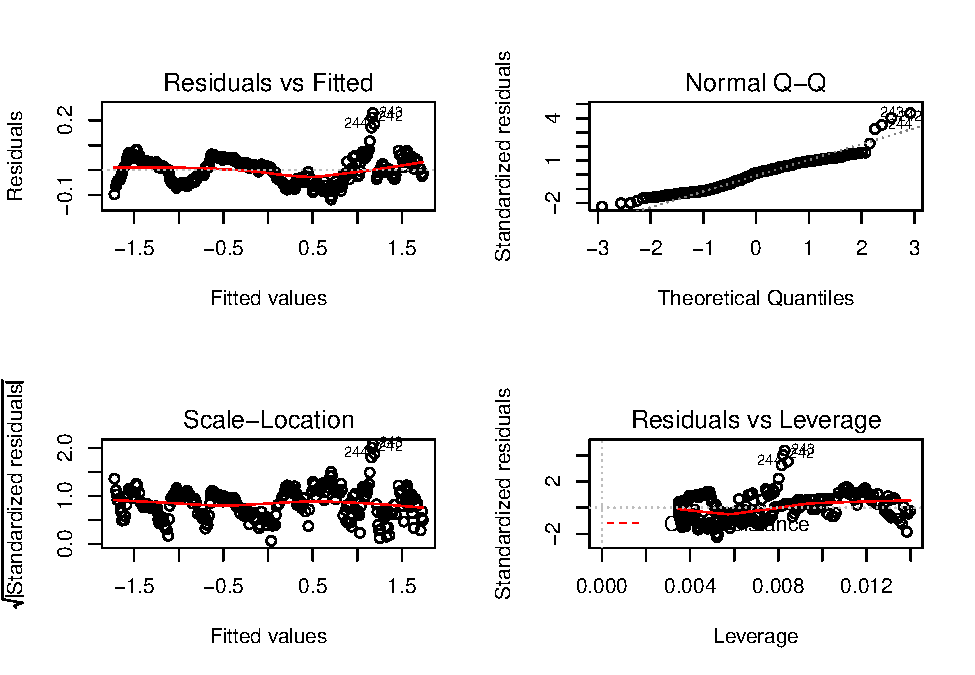
\includegraphics{Lab9_files/figure-latex/unnamed-chunk-10-1.pdf}

\begin{Shaded}
\begin{Highlighting}[]
\NormalTok{m_bty <-}\StringTok{ }\KeywordTok{lm}\NormalTok{(evals}\OperatorTok{$}\NormalTok{score }\OperatorTok{~}\StringTok{ }\NormalTok{evals}\OperatorTok{$}\NormalTok{bty_avg)}
\KeywordTok{summary}\NormalTok{(m_bty)}
\end{Highlighting}
\end{Shaded}

\begin{verbatim}
## 
## Call:
## lm(formula = evals$score ~ evals$bty_avg)
## 
## Residuals:
##     Min      1Q  Median      3Q     Max 
## -1.9246 -0.3690  0.1420  0.3977  0.9309 
## 
## Coefficients:
##               Estimate Std. Error t value Pr(>|t|)    
## (Intercept)    3.88034    0.07614   50.96  < 2e-16 ***
## evals$bty_avg  0.06664    0.01629    4.09 5.08e-05 ***
## ---
## Signif. codes:  0 '***' 0.001 '**' 0.01 '*' 0.05 '.' 0.1 ' ' 1
## 
## Residual standard error: 0.5348 on 461 degrees of freedom
## Multiple R-squared:  0.03502,    Adjusted R-squared:  0.03293 
## F-statistic: 16.73 on 1 and 461 DF,  p-value: 5.083e-05
\end{verbatim}

Let's see if the apparent trend in the plot is something more than
natural variation. Fit a linear model called m\_bty to predict average
professor score by average beauty rating. Write out the equation for the
linear model and interpret the slope. Is average beauty score a
statistically significant predictor? Does it appear to be a practically
significant predictor?

The equation for the linear model is:

\[y = 3.88034 + 0.06664\]

Where y is the predicted score of the professor based on x, the average
beauty of the professor.

In this case, the slope is slightly positive at 0.067 and it indicates
that as beauty increases the average score of professors on evaluations
also increases marginally.

Based on the low r-squared values (both adjusted and predicted) and the
low p-value, it appears as though average beauty is not a practically
significant predictor of evaluation score. The low r-squared values
indicate that another model may be suited for prediction. Though the low
p-value indicates that the relationship between these variables is
statistically significant at a level of 0.001.

\hypertarget{exercise-6}{%
\subsubsection{Exercise 6}\label{exercise-6}}

Use residual plots to evaluate whether the conditions of least squares
regression are reasonable. Provide plots and comments for each one (see
the Simple Regression Lab for a reminder of how to make these).

\begin{Shaded}
\begin{Highlighting}[]
\KeywordTok{hist}\NormalTok{(m_bty}\OperatorTok{$}\NormalTok{residuals)}
\end{Highlighting}
\end{Shaded}

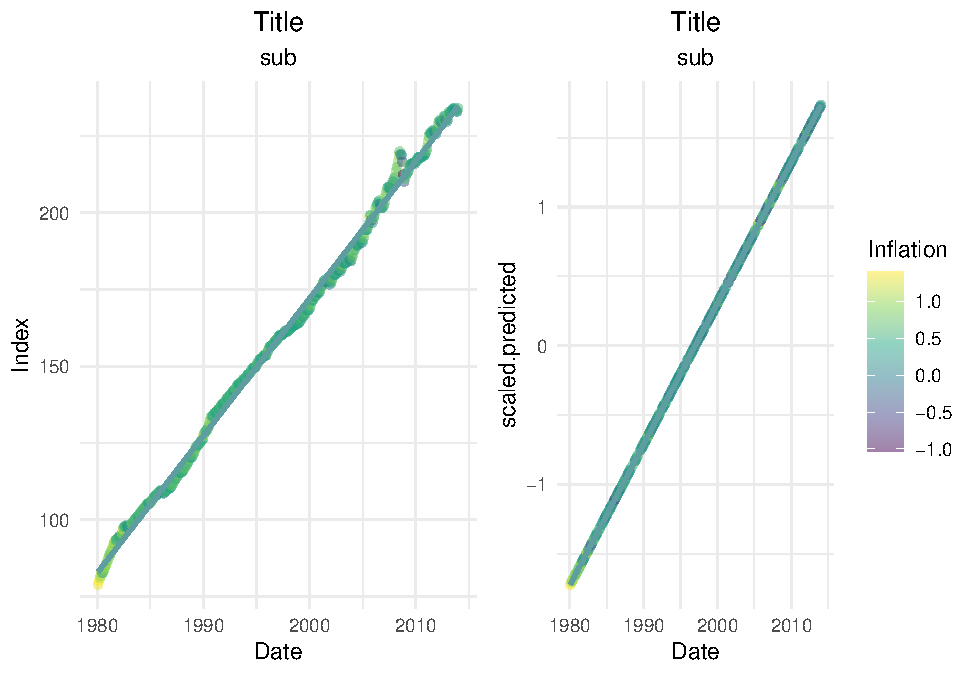
\includegraphics{Lab9_files/figure-latex/unnamed-chunk-12-1.pdf}

A histogram shows the distribution of the residuals to be left skewed
and not normally distributed.

\begin{Shaded}
\begin{Highlighting}[]
\KeywordTok{plot}\NormalTok{(m_bty}\OperatorTok{$}\NormalTok{residuals }\OperatorTok{~}\StringTok{ }\NormalTok{evals}\OperatorTok{$}\NormalTok{bty_avg, }\DataTypeTok{ylab=}\StringTok{"Residuals"}\NormalTok{, }\DataTypeTok{xlab=}\StringTok{"Average Beauty"}\NormalTok{, }
\DataTypeTok{main=}\StringTok{"Rating and Beauty"}\NormalTok{) }
\KeywordTok{abline}\NormalTok{(}\DataTypeTok{h =} \DecValTok{0}\NormalTok{, }\DataTypeTok{lty =} \DecValTok{3}\NormalTok{)  }\CommentTok{# adds a horizontal dashed line at y = 0}
\end{Highlighting}
\end{Shaded}

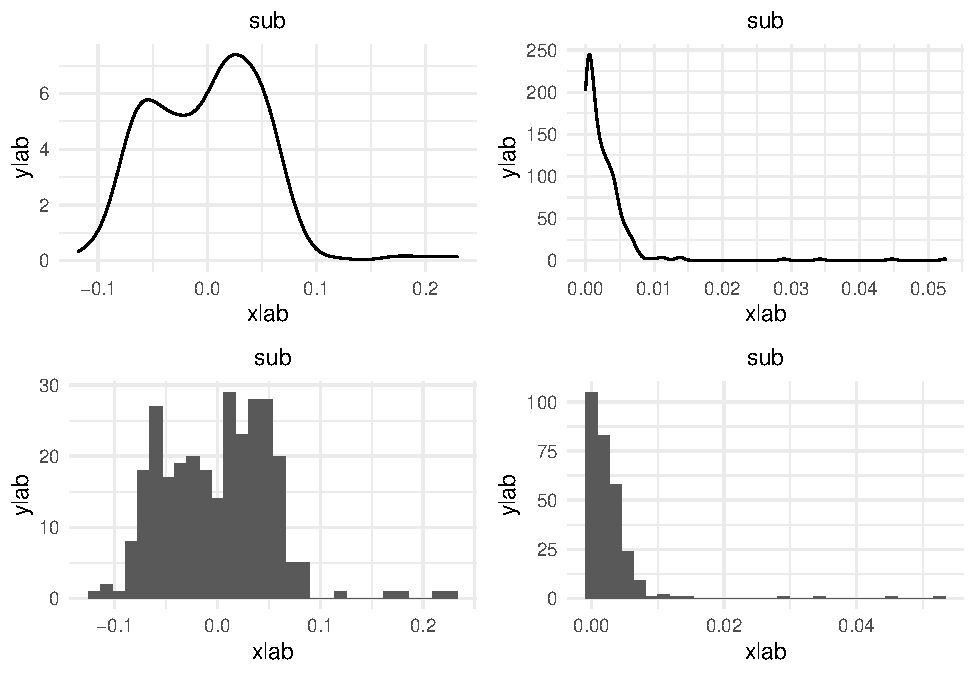
\includegraphics{Lab9_files/figure-latex/unnamed-chunk-13-1.pdf}

This scatterplot fo the residuals also shows the distribution to be left
skewed and not normally distributed. The residuals are not constantly
variable around the zero line. They are concentrated to the right and
might not follow a linear trend.

\hypertarget{exercise-7}{%
\subsubsection{Exercise 7}\label{exercise-7}}

P-values and parameter estimates should only be trusted if the
conditions for the regression are reasonable. Verify that the conditions
for this model are reasonable using diagnostic plots.

\begin{Shaded}
\begin{Highlighting}[]
\KeywordTok{ggplot}\NormalTok{(}\DataTypeTok{data =}\NormalTok{ evals, }\KeywordTok{aes}\NormalTok{(}\DataTypeTok{x =}\NormalTok{ bty_f1lower, }\DataTypeTok{y =}\NormalTok{ bty_avg)) }\OperatorTok{+}
\StringTok{  }\KeywordTok{geom_point}\NormalTok{()}
\end{Highlighting}
\end{Shaded}

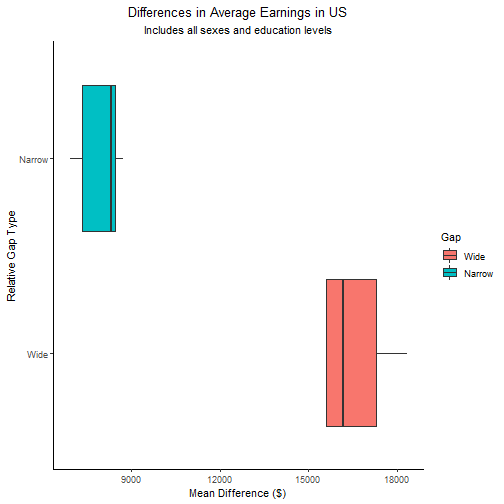
\includegraphics{Lab9_files/figure-latex/unnamed-chunk-14-1.pdf}

\begin{Shaded}
\begin{Highlighting}[]
\NormalTok{evals }\OperatorTok\StringTok{ }
\StringTok{  }\KeywordTok{summarise}\NormalTok{(}\KeywordTok{cor}\NormalTok{(bty_avg, bty_f1lower))}
\end{Highlighting}
\end{Shaded}

\begin{verbatim}
## # A tibble: 1 x 1
##   `cor(bty_avg, bty_f1lower)`
##                         <dbl>
## 1                       0.844
\end{verbatim}

\begin{Shaded}
\begin{Highlighting}[]
\NormalTok{evals }\OperatorTok
\StringTok{  }\KeywordTok{select}\NormalTok{(}\KeywordTok{contains}\NormalTok{(}\StringTok{"bty"}\NormalTok{)) }\OperatorTok
\StringTok{  }\KeywordTok{ggpairs}\NormalTok{()}
\end{Highlighting}
\end{Shaded}

\includegraphics{Lab9_files/figure-latex/unnamed-chunk-14-2.pdf}

\begin{Shaded}
\begin{Highlighting}[]
\NormalTok{m_bty_gen <-}\StringTok{ }\KeywordTok{lm}\NormalTok{(score }\OperatorTok{~}\StringTok{ }\NormalTok{bty_avg }\OperatorTok{+}\StringTok{ }\NormalTok{gender, }\DataTypeTok{data =}\NormalTok{ evals)}
\KeywordTok{summary}\NormalTok{(m_bty_gen)}
\end{Highlighting}
\end{Shaded}

\begin{verbatim}
## 
## Call:
## lm(formula = score ~ bty_avg + gender, data = evals)
## 
## Residuals:
##     Min      1Q  Median      3Q     Max 
## -1.8305 -0.3625  0.1055  0.4213  0.9314 
## 
## Coefficients:
##             Estimate Std. Error t value Pr(>|t|)    
## (Intercept)  3.74734    0.08466  44.266  < 2e-16 ***
## bty_avg      0.07416    0.01625   4.563 6.48e-06 ***
## gendermale   0.17239    0.05022   3.433 0.000652 ***
## ---
## Signif. codes:  0 '***' 0.001 '**' 0.01 '*' 0.05 '.' 0.1 ' ' 1
## 
## Residual standard error: 0.5287 on 460 degrees of freedom
## Multiple R-squared:  0.05912,    Adjusted R-squared:  0.05503 
## F-statistic: 14.45 on 2 and 460 DF,  p-value: 8.177e-07
\end{verbatim}

The conditions for least squares regression are:

\begin{verbatim}
* Linearity
* ~ Normal Residuals
* Constant Variability
* Independent Observations
\end{verbatim}

These describe that the data should display linear trends, have nearly
normal residuals with constant variability, and each observation should
be independent of the other observations.

\begin{Shaded}
\begin{Highlighting}[]
\KeywordTok{qqnorm}\NormalTok{(m_bty_gen}\OperatorTok{$}\NormalTok{residuals)}
\KeywordTok{qqline}\NormalTok{(m_bty_gen}\OperatorTok{$}\NormalTok{residuals)}
\end{Highlighting}
\end{Shaded}

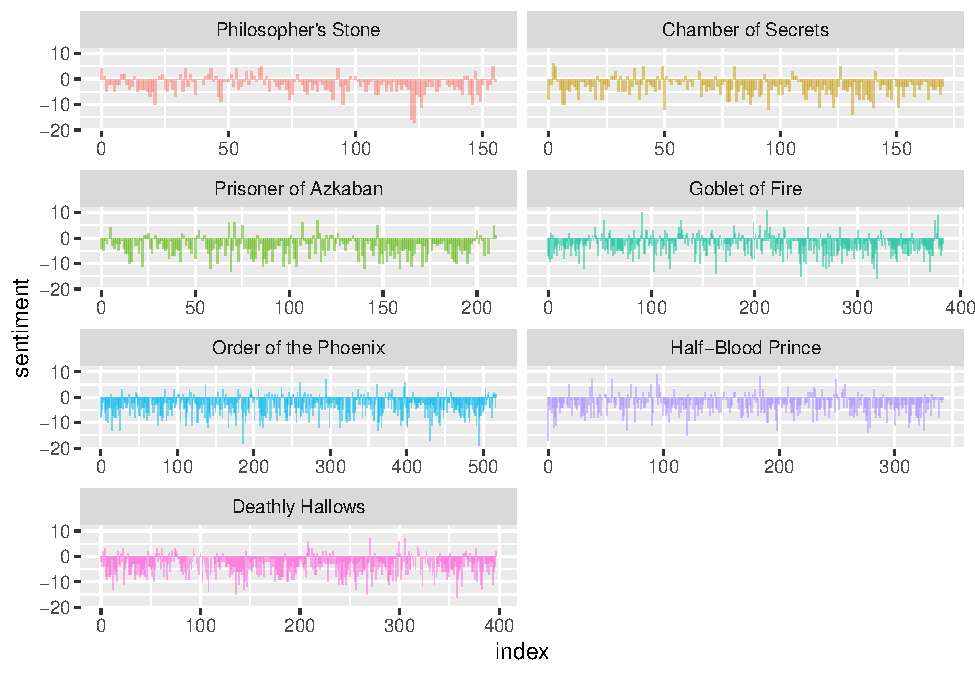
\includegraphics{Lab9_files/figure-latex/unnamed-chunk-16-1.pdf}

We can be confident that the observations are independent of one
another. However, given that the residuals are not normal all of these
conditions are not met. It may also be the case that the data do not fit
a linear model.

\hypertarget{exercise-8}{%
\subsubsection{Exercise 8}\label{exercise-8}}

Is bty\_avg still a significant predictor of score? Has the addition of
gender to the model changed the parameter estimate for gender?

Yes, there was a marginal increase in the intercept and slope but not
enough to have a significant change on bty\_avg as a significant
predictor of score.

\hypertarget{exercise-9}{%
\subsubsection{Exercise 9}\label{exercise-9}}

What is the equation of the line corresponding to males? (Hint: For
males, the parameter estimate is multiplied by 1.) For two professors
who received the same beauty rating, which gender tends to have the
higher course evaluation score?

The equation of the line corresponding to males is

\[score = 3.74734 + 0.07416(b) + 0.17239(m) \] where b is the b is the
average beauty rating and m is the classifier ``1'' given to males. For
females we would use the variable f which is classified as a 0.

Males tend to have a higher course evaluation score.

\hypertarget{exercise-10}{%
\subsubsection{Exercise 10}\label{exercise-10}}

Create a new model called m\_bty\_rank with gender removed and rank
added in. How does R appear to handle categorical variables that have
more than two levels? Note that the rank variable has three levels:
teaching, tenure track, tenured.

\begin{Shaded}
\begin{Highlighting}[]
\NormalTok{m_bty_rank <-}\StringTok{ }\KeywordTok{lm}\NormalTok{(score }\OperatorTok{~}\StringTok{ }\NormalTok{bty_avg }\OperatorTok{+}\StringTok{ }\NormalTok{rank, }\DataTypeTok{data =}\NormalTok{ evals)}
\KeywordTok{summary}\NormalTok{(m_bty_rank)}
\end{Highlighting}
\end{Shaded}

\begin{verbatim}
## 
## Call:
## lm(formula = score ~ bty_avg + rank, data = evals)
## 
## Residuals:
##     Min      1Q  Median      3Q     Max 
## -1.8713 -0.3642  0.1489  0.4103  0.9525 
## 
## Coefficients:
##                  Estimate Std. Error t value Pr(>|t|)    
## (Intercept)       3.98155    0.09078  43.860  < 2e-16 ***
## bty_avg           0.06783    0.01655   4.098 4.92e-05 ***
## ranktenure track -0.16070    0.07395  -2.173   0.0303 *  
## ranktenured      -0.12623    0.06266  -2.014   0.0445 *  
## ---
## Signif. codes:  0 '***' 0.001 '**' 0.01 '*' 0.05 '.' 0.1 ' ' 1
## 
## Residual standard error: 0.5328 on 459 degrees of freedom
## Multiple R-squared:  0.04652,    Adjusted R-squared:  0.04029 
## F-statistic: 7.465 on 3 and 459 DF,  p-value: 6.88e-05
\end{verbatim}

Since only two categorical variables appear in the results of the linear
regression, I would assume that R is purposefully excluding one of the
three categories. In this case, the missing category is teaching.

\hypertarget{exercise-11}{%
\subsubsection{Exercise 11}\label{exercise-11}}

Which variable would you expect to have the highest p-value in this
model? Why? Hint: Think about which variable would you expect to not
have any association with the professor score.

The variable that should be the least likely to have any association
with the professor score is the cls\_level. In this case, the level of
the class as upper or lower should not have any association with the
professor score. Additionally, there is often overlap in upper and lower
level courses for all students.

\hypertarget{exercise-12}{%
\subsubsection{Exercise 12}\label{exercise-12}}

Check your suspicions from the previous exercise. Include the model
output in your response.

\begin{Shaded}
\begin{Highlighting}[]
\NormalTok{m_full <-}\StringTok{ }\KeywordTok{lm}\NormalTok{(score }\OperatorTok{~}\StringTok{ }\NormalTok{rank }\OperatorTok{+}\StringTok{ }\NormalTok{gender }\OperatorTok{+}\StringTok{ }\NormalTok{ethnicity }\OperatorTok{+}\StringTok{ }\NormalTok{language }\OperatorTok{+}\StringTok{ }\NormalTok{age }\OperatorTok{+}\StringTok{ }\NormalTok{cls_perc_eval }
             \OperatorTok{+}\StringTok{ }\NormalTok{cls_students }\OperatorTok{+}\StringTok{ }\NormalTok{cls_level }\OperatorTok{+}\StringTok{ }\NormalTok{cls_profs }\OperatorTok{+}\StringTok{ }\NormalTok{cls_credits }\OperatorTok{+}\StringTok{ }\NormalTok{bty_avg }
             \OperatorTok{+}\StringTok{ }\NormalTok{pic_outfit }\OperatorTok{+}\StringTok{ }\NormalTok{pic_color, }\DataTypeTok{data =}\NormalTok{ evals)}
\KeywordTok{summary}\NormalTok{(m_full)}
\end{Highlighting}
\end{Shaded}

\begin{verbatim}
## 
## Call:
## lm(formula = score ~ rank + gender + ethnicity + language + age + 
##     cls_perc_eval + cls_students + cls_level + cls_profs + cls_credits + 
##     bty_avg + pic_outfit + pic_color, data = evals)
## 
## Residuals:
##      Min       1Q   Median       3Q      Max 
## -1.77397 -0.32432  0.09067  0.35183  0.95036 
## 
## Coefficients:
##                         Estimate Std. Error t value Pr(>|t|)    
## (Intercept)            4.0952141  0.2905277  14.096  < 2e-16 ***
## ranktenure track      -0.1475932  0.0820671  -1.798  0.07278 .  
## ranktenured           -0.0973378  0.0663296  -1.467  0.14295    
## gendermale             0.2109481  0.0518230   4.071 5.54e-05 ***
## ethnicitynot minority  0.1234929  0.0786273   1.571  0.11698    
## languagenon-english   -0.2298112  0.1113754  -2.063  0.03965 *  
## age                   -0.0090072  0.0031359  -2.872  0.00427 ** 
## cls_perc_eval          0.0053272  0.0015393   3.461  0.00059 ***
## cls_students           0.0004546  0.0003774   1.205  0.22896    
## cls_levelupper         0.0605140  0.0575617   1.051  0.29369    
## cls_profssingle       -0.0146619  0.0519885  -0.282  0.77806    
## cls_creditsone credit  0.5020432  0.1159388   4.330 1.84e-05 ***
## bty_avg                0.0400333  0.0175064   2.287  0.02267 *  
## pic_outfitnot formal  -0.1126817  0.0738800  -1.525  0.12792    
## pic_colorcolor        -0.2172630  0.0715021  -3.039  0.00252 ** 
## ---
## Signif. codes:  0 '***' 0.001 '**' 0.01 '*' 0.05 '.' 0.1 ' ' 1
## 
## Residual standard error: 0.498 on 448 degrees of freedom
## Multiple R-squared:  0.1871, Adjusted R-squared:  0.1617 
## F-statistic: 7.366 on 14 and 448 DF,  p-value: 6.552e-14
\end{verbatim}

My assumption was incorrect. Cls\_profs had the highest p-value and thus
the least likely association with score. This categorical variable
observes whether the course had multiple professors teaching sections in
the course or if there was only a single professor teaching all sections
for the course. It turns out that this has little to no influence on the
professor score.

\hypertarget{exercise-13}{%
\subsubsection{Exercise 13}\label{exercise-13}}

Interpret the coefficient associated with the ethnicity variable.

Holding all other variables constant, we would expect that a
non-minority professor would rate about 0.1235 points higher on their
evaluations. However, given the large p-value the results would not be
significant as there is a poor association between the professor's
ethnicity and the professor's score.

\hypertarget{exercise-14}{%
\subsubsection{Exercise 14}\label{exercise-14}}

Drop the variable with the highest p-value and re-fit the model. Did the
coefficients and significance of the other explanatory variables change?
(One of the things that makes multiple regression interesting is that
coefficient estimates depend on the other variables that are included in
the model.) If not, what does this say about whether or not the dropped
variable was collinear with the other explanatory variables?

\begin{Shaded}
\begin{Highlighting}[]
\NormalTok{m_full_drop1 <-}\StringTok{ }\KeywordTok{lm}\NormalTok{(score }\OperatorTok{~}\StringTok{ }\NormalTok{rank }\OperatorTok{+}\StringTok{ }\NormalTok{gender }\OperatorTok{+}\StringTok{ }\NormalTok{ethnicity }\OperatorTok{+}\StringTok{ }\NormalTok{language }\OperatorTok{+}\StringTok{ }\NormalTok{age }\OperatorTok{+}\StringTok{ }\NormalTok{cls_perc_eval }
             \OperatorTok{+}\StringTok{ }\NormalTok{cls_students }\OperatorTok{+}\StringTok{ }\NormalTok{cls_level }\OperatorTok{+}\StringTok{ }\NormalTok{cls_credits }\OperatorTok{+}\StringTok{ }\NormalTok{bty_avg }
             \OperatorTok{+}\StringTok{ }\NormalTok{pic_outfit }\OperatorTok{+}\StringTok{ }\NormalTok{pic_color, }\DataTypeTok{data =}\NormalTok{ evals)}
\KeywordTok{summary}\NormalTok{(m_full_drop1)}
\end{Highlighting}
\end{Shaded}

\begin{verbatim}
## 
## Call:
## lm(formula = score ~ rank + gender + ethnicity + language + age + 
##     cls_perc_eval + cls_students + cls_level + cls_credits + 
##     bty_avg + pic_outfit + pic_color, data = evals)
## 
## Residuals:
##     Min      1Q  Median      3Q     Max 
## -1.7836 -0.3257  0.0859  0.3513  0.9551 
## 
## Coefficients:
##                         Estimate Std. Error t value Pr(>|t|)    
## (Intercept)            4.0872523  0.2888562  14.150  < 2e-16 ***
## ranktenure track      -0.1476746  0.0819824  -1.801 0.072327 .  
## ranktenured           -0.0973829  0.0662614  -1.470 0.142349    
## gendermale             0.2101231  0.0516873   4.065 5.66e-05 ***
## ethnicitynot minority  0.1274458  0.0772887   1.649 0.099856 .  
## languagenon-english   -0.2282894  0.1111305  -2.054 0.040530 *  
## age                   -0.0089992  0.0031326  -2.873 0.004262 ** 
## cls_perc_eval          0.0052888  0.0015317   3.453 0.000607 ***
## cls_students           0.0004687  0.0003737   1.254 0.210384    
## cls_levelupper         0.0606374  0.0575010   1.055 0.292200    
## cls_creditsone credit  0.5061196  0.1149163   4.404 1.33e-05 ***
## bty_avg                0.0398629  0.0174780   2.281 0.023032 *  
## pic_outfitnot formal  -0.1083227  0.0721711  -1.501 0.134080    
## pic_colorcolor        -0.2190527  0.0711469  -3.079 0.002205 ** 
## ---
## Signif. codes:  0 '***' 0.001 '**' 0.01 '*' 0.05 '.' 0.1 ' ' 1
## 
## Residual standard error: 0.4974 on 449 degrees of freedom
## Multiple R-squared:  0.187,  Adjusted R-squared:  0.1634 
## F-statistic: 7.943 on 13 and 449 DF,  p-value: 2.336e-14
\end{verbatim}

Yes, there were slight changes in the the coefficients and significance
of the other explanatory variables.

\hypertarget{exercise-15}{%
\subsubsection{Exercise 15}\label{exercise-15}}

Using backward-selection and p-value as the selection criterion,
determine the best model. You do not need to show all steps in your
answer, just the output for the final model. Also, write out the linear
model for predicting score based on the final model you settle on.

\begin{Shaded}
\begin{Highlighting}[]
\NormalTok{m_full_best <-}\StringTok{ }\KeywordTok{lm}\NormalTok{(score }\OperatorTok{~}\StringTok{ }\NormalTok{gender }
                  \OperatorTok{+}\StringTok{ }\NormalTok{ethnicity }
                  \OperatorTok{+}\StringTok{ }\NormalTok{age }
                  \OperatorTok{+}\StringTok{ }\NormalTok{language}
                  \OperatorTok{+}\StringTok{ }\NormalTok{cls_perc_eval }
              \OperatorTok{+}\StringTok{ }\NormalTok{cls_credits }
              \OperatorTok{+}\StringTok{ }\NormalTok{bty_avg }
             \OperatorTok{+}\StringTok{ }\NormalTok{pic_color, }\DataTypeTok{data =}\NormalTok{ evals)}
\KeywordTok{summary}\NormalTok{(m_full_best)}
\end{Highlighting}
\end{Shaded}

\begin{verbatim}
## 
## Call:
## lm(formula = score ~ gender + ethnicity + age + language + cls_perc_eval + 
##     cls_credits + bty_avg + pic_color, data = evals)
## 
## Residuals:
##      Min       1Q   Median       3Q      Max 
## -1.85320 -0.32394  0.09984  0.37930  0.93610 
## 
## Coefficients:
##                        Estimate Std. Error t value Pr(>|t|)    
## (Intercept)            3.771922   0.232053  16.255  < 2e-16 ***
## gendermale             0.207112   0.050135   4.131 4.30e-05 ***
## ethnicitynot minority  0.167872   0.075275   2.230  0.02623 *  
## age                   -0.006046   0.002612  -2.315  0.02108 *  
## languagenon-english   -0.206178   0.103639  -1.989  0.04726 *  
## cls_perc_eval          0.004656   0.001435   3.244  0.00127 ** 
## cls_creditsone credit  0.505306   0.104119   4.853 1.67e-06 ***
## bty_avg                0.051069   0.016934   3.016  0.00271 ** 
## pic_colorcolor        -0.190579   0.067351  -2.830  0.00487 ** 
## ---
## Signif. codes:  0 '***' 0.001 '**' 0.01 '*' 0.05 '.' 0.1 ' ' 1
## 
## Residual standard error: 0.4992 on 454 degrees of freedom
## Multiple R-squared:  0.1722, Adjusted R-squared:  0.1576 
## F-statistic:  11.8 on 8 and 454 DF,  p-value: 2.58e-15
\end{verbatim}

The best linear model for predicting score based on backward-selection
and p-value significance is:

\[score = 3.771922+0.207112(gender)+0.167872(ethnicity)-0.006046(age) - 0.206178(language) \n +0.004656(cls_perc_eval)+ 0.505306(cls_credits)+ 0.051069(bty_avg)-0.190579 (pic_color)\]

\hypertarget{exercise-16}{%
\subsubsection{Exercise 16}\label{exercise-16}}

\hypertarget{exercise-17}{%
\subsubsection{Exercise 17}\label{exercise-17}}

\hypertarget{exercise-18}{%
\subsubsection{Exercise 18}\label{exercise-18}}

\hypertarget{exercise-19}{%
\subsubsection{Exercise 19}\label{exercise-19}}

\ldots{}

\end{document}
